



\begin{figure}[t]
   \centering

%   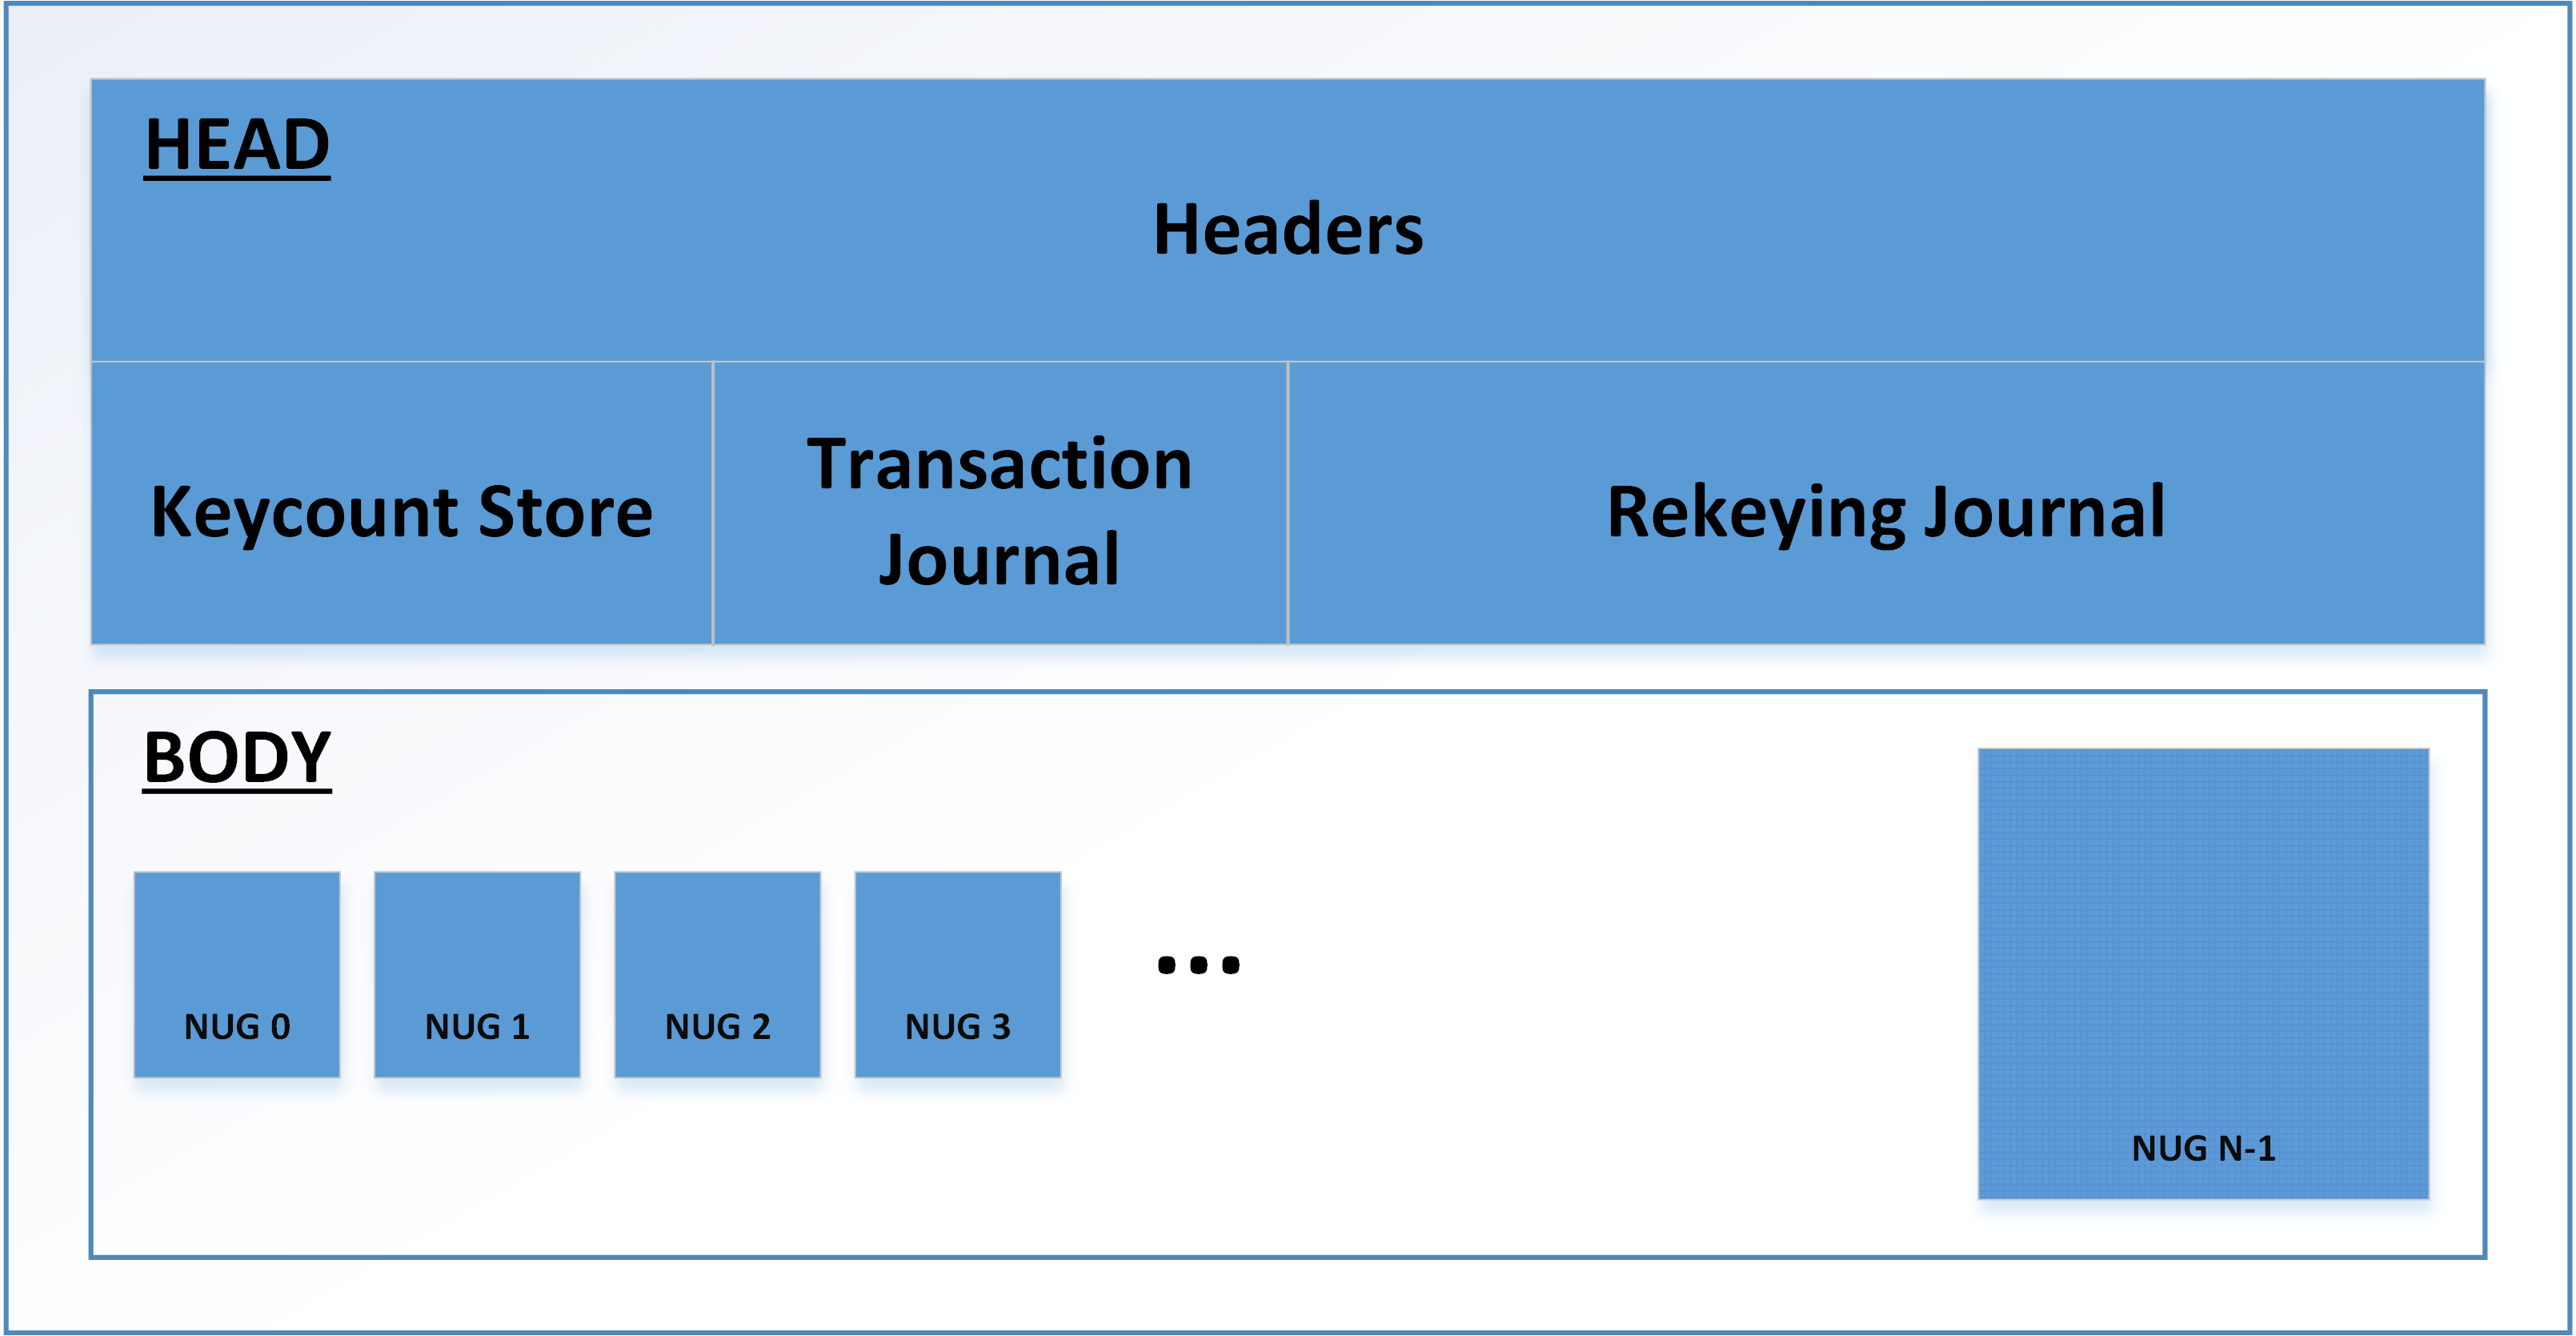
\includegraphics[width=\linewidth]{backstore.png}

   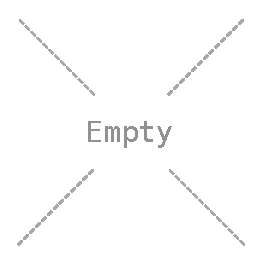
\includegraphics[height=1in]{empty.eps}

   \mycaption{fig:backstore}{Layout of SwitchCrypt's drive layout.}{The figure is explained
in Section \ref{..}.}

\end{figure}


\section{Overview} 
\label{subsec:overview}




SwitchCrypt consists of a \emph{Generic Stream Cipher Interface} and
\emph{Cryptographic Driver}; SwitchCrypt sits between a Log-structured File
System (LFS) on the OS, and the underlying drive (backing storage) and device
controller (e.g. Flash Translation Layer). This is illustrated in
\figref{overview}, which provides an overview of the SwitchCrypt system design.


The drive itself is divided into a \emph{HEAD} section and \emph{BODY} section
upon initialization, illustrated in \figref{backstore}. The HEAD consists of
metadata headers written during initialization~\cite{StrongBox} along with the
\emph{Keycount Store}, \emph{Transaction Journal}, \emph{Rekeying Journal}, and
\emph{Per-Nugget Metadata}, each drive-backed. These components are used by the
\emph{Cryptographic Driver} together with the \emph{Cipher Switching Strategy}
implementations to enable efficient per-unit cipher switching.

The BODY consists of a series independent same-size logical units called
\emph{nuggets}. A nugget consists of one or more contiguous physical drive
blocks. Each nugget is coupled with metadata in the HEAD indicating which cipher
was used to encrypt the nugget along with any additional ciphertext output; the
latter allows us to treat any non-length-preserving ciphers as if they were
length-preserving. SwitchCrypt uses the Keycount Store and Transaction Journal
components along with our nugget layout to 1) track, detect, and handle
overwrites, 2) limit the maximum length of any plaintext input to ciphers, thus
amortizing the overhead incurred during encryption, and 3) independently and
efficiently switch the cipher used to encrypt individual nuggets.

Dickens et al. showed how to make nugget-based drive organization secure using a
single stream cipher, ChaCha20, to handle overwrites, prevent rollback attacks,
and limit plaintext length~\cite{StrongBox}. However, they did not envision the
utility in trading off between concerns at the filesystem or device-mapper
level, dynamic cipher switching, or protecting against attacks on data ``in
motion;'' the remainder of this section details the novel components that enable
this functionality. Specifically: how we quantify the properties traded off
between configurations (\cref{subsec:quantify}), the Generic Stream Cipher
Interface and Per-Nugget Metadata components (\cref{subsec:interface}) which
decouple cipher implementations from the encryption process, and our Cipher
Switching Strategy implementations (\cref{subsec:strategies}) used to
efficiently encrypt nuggets with different ciphers.
